\graphicspath{{7ren/pics/}}

\section{The Renaissance in Europe}

\subsection{Fibonacci and Notational Development}

Between the fall of Rome in 476 and the early renaissance\footnote{Literally \emph{rebirth.} Dates vary by location and discipline (Italy vs.{} France, art vs.{} philosophy, etc.) but a wide net would encompass the 12\th{} to 17\th{} centuries.} (c.\,1100) came Europe's dark ages. The one-dimensional view is that this was a time of limited learning and technological progress; as ever, the reality was more complex. Learning persisted in monasteries, though new researches took second place to a conservative focus on preserving the wisdom of the ancients.\smallbreak
By 1100, the small shifting kingdoms that had characterised Europe were starting to come together as more stable feudal states.\footnote{An arrangement where powerful landowners could demand service (rent, food, warriors) from their tenants.} The maps below show the major feudal societies of medieval Europe (France, England, Holy Roman Empire, Poland, Austria) consolidating. While it would have meant little to the average peasant, a large stable nation is able to produce and support a larger elite population with the time and money to pursue education, and fund libraries and universities. By the 1700s, the borders of western Europe are largely recognizable; political and social organization had expanded so that a much larger proportion of the population---though small in comparison to today---were able to take advantage of and contribute to the growth of knowledge. The European renaissance is often contrasted with a decline in Islamic power, but again the story is more complex: Islam retreats from Spain, while the Ottoman Empire becomes dominant in south-east Europe.

\begin{center}
	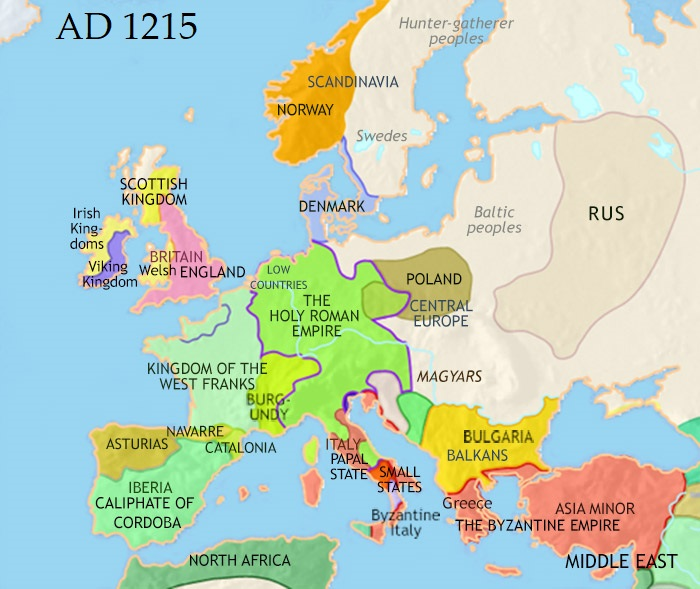
\includegraphics[width=0.32\linewidth]{europe1215} \
	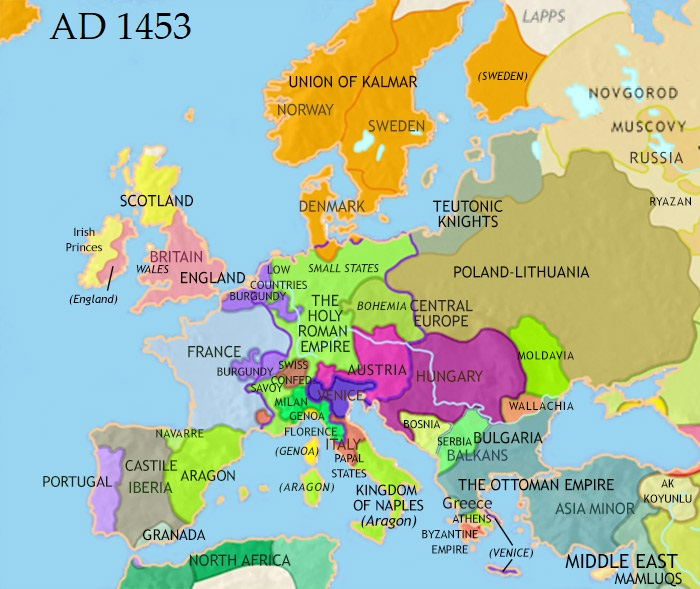
\includegraphics[width=0.32\linewidth]{europe1453} \
	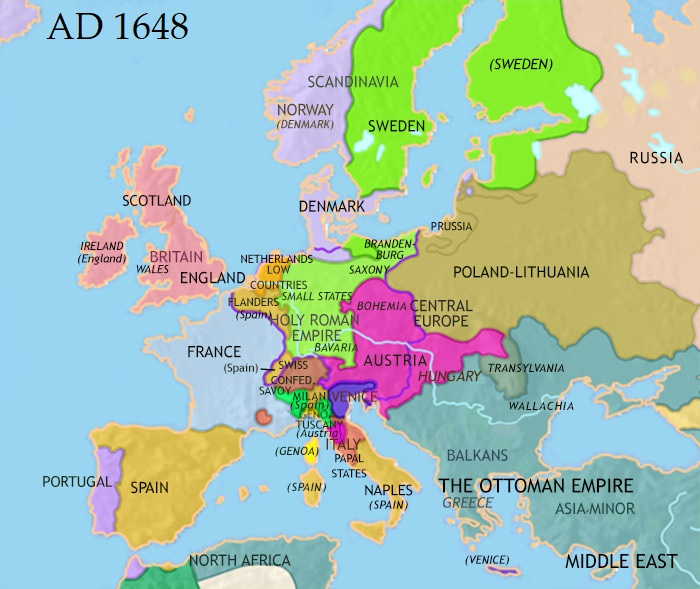
\includegraphics[width=0.32\linewidth]{europe1648}
\end{center}

Between 900 and 1300, the population of Europe roughly tripled to around 100 million. Trade increased, along with which came knowledge.\footnote{A particularly important trading hub was Venice, from where Marco Polo (1254--1324), perhaps the most famous trader of the period, travelled the silk road to China.} Learning (and land) came via wars with Islam (the Crusades, Spain, etc.). It helped that Islamic scholars so venerated the Greeks; Europeans could tell themselves that they were merely `reclaiming' ancient knowledge which had been `stolen' by their cultural and religious enemies. The fall of Constantinople to Mehmet in 1453 marks both the high point of Islamic conquest and the start of the decline of Islamic scientific dominance. Many intellectuals fled Constantinople---where the Byzantines still preserved much of Alexandria's learning---for Rome, helping to further fuel developments. With powerful enemies to the east, Europeans began travelling greater distances by sea,\footnote{Christopher Columbus (born Genoa 1451) famously `discovered' America in 1492 while looking for sea routes to Asia.} beginning the colonial era of global European empire.
\goodbreak



%\boldsubsubsection{Education in the Renaissance}

Scientific and philosophical progress was spurred by the translation of works from Arabic and ancient Greek into Latin, with the first universities being formed to teach this canon: Bologna 1088, Paris 1150, and Oxford 1167. The typical student was a young man of wealth who had been privately tutored in grammar, logic \& rhetoric (the \emph{trivium}). At university he would study the Greek-influenced \emph{quadrivium} (geometry, astronomy, arithmetic \& music). While Islamic improvements were incorporated, scholars gave pre-eminence to the Greeks: Euclid for geometry, Aristotle for logic/physics, Hippocrates/Galen for medicine, Ptolemy for astronomy. Early universities were often funded by the Church and `research' was more likely to involve the justification of biblical passages using Aristotle than the conduct of experiments.


\boldinline{Leonardo da Pisa (Fibonacci c.\,1175--1250)}

Fibonacci\footnote{The name was given to Leonardo by French scholars of the 1800s: \emph{filius Bonacci} means \emph{son of Bonacci.}} likely first encountered the Hindu--Arabic numerals while trading with his father in North Africa. He was impressed by the ease of calculation they afforded and is the first European known to use them (contemporary Europeans used Roman numerals and Egyptian fractions). Fibonacci's 1202 text \emph{Liber Abaci} was written to instruct traders in their use. The first page below explains how to compute with decimal fractions, with the two columns at the bottom of the page showing how to repeatedly multiply 100 (and then 10) by the fraction $\frac 9{10}$. Thus:
\[
	100,\quad 90,\quad 81,\quad \frac 9{10}72\ (=72.9),\quad \frac 1{10}\!\frac 6{10}65\ (=65.61),\quad\frac 9{10}\!\frac 4{10}\!\frac 0{10}59\ (=59.049),\quad\text{etc.}
\]
\begin{center}
	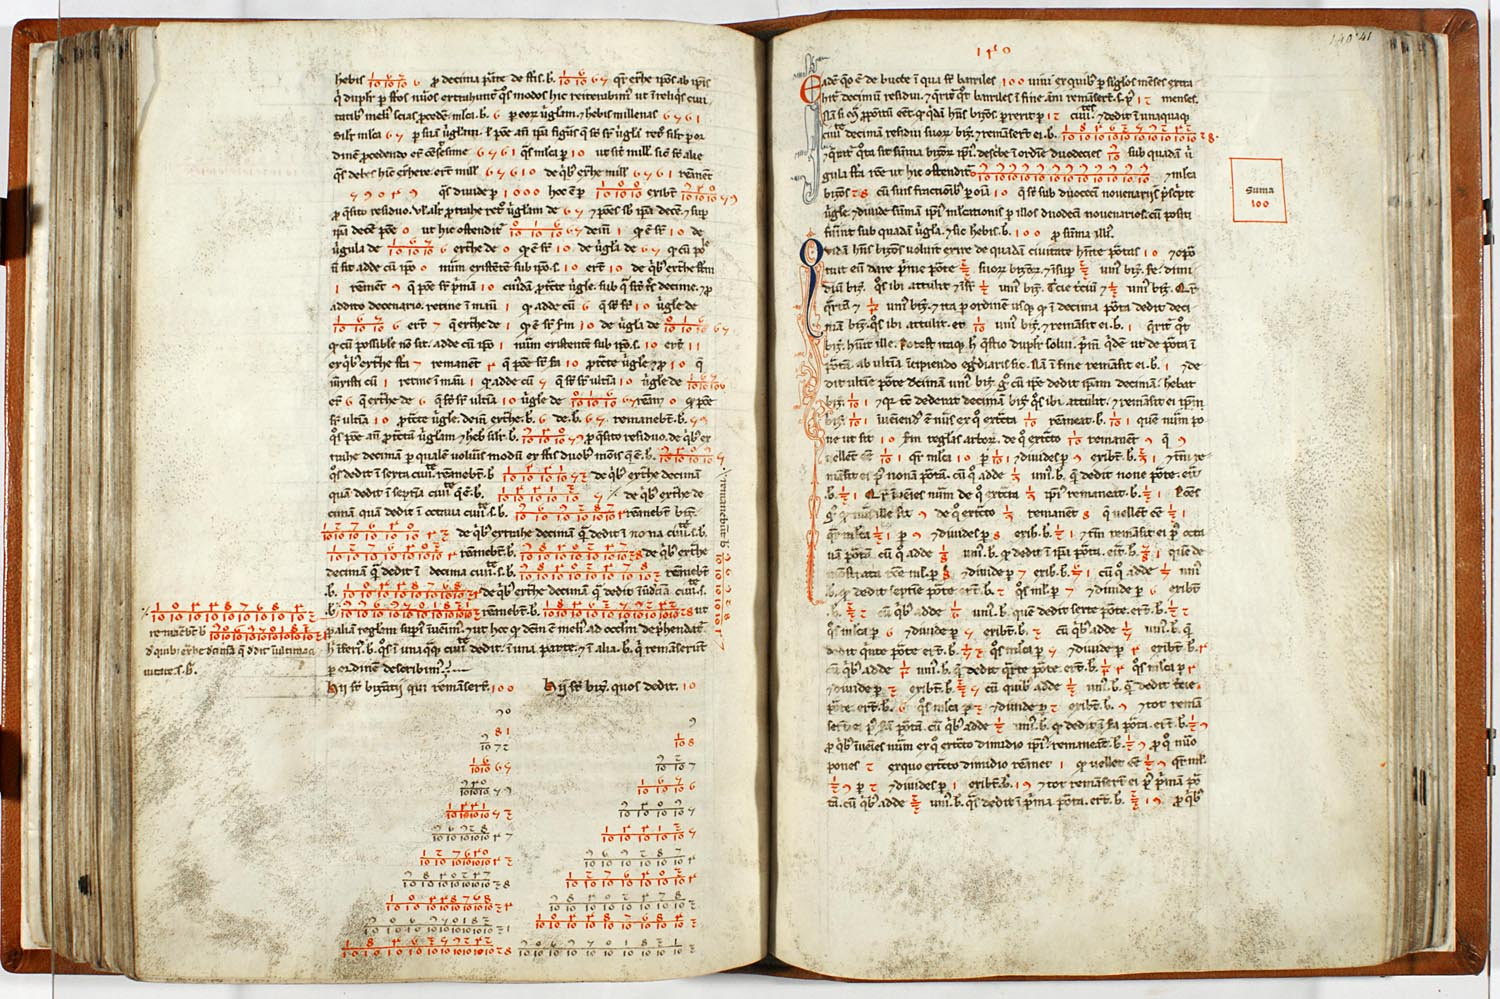
\includegraphics[height=250pt]{liberabaci3}
	\quad
	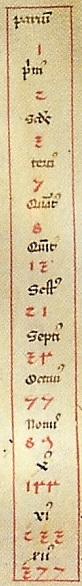
\includegraphics[height=250pt]{liberabaci1}
\end{center}
Note how the fractional part is written backwards on the left, using a bar to separate numerator and denominator; the Indians wrote fractions without a bar and it is thought Islamic scholars inserted it for clarity in the 1100s. The second picture is of Fibonacci's famous sequence: read top-to-bottom 1, 2, 3, 5, 8, 13, 21, 34, 55, 89, 144, 233, 377. Amongst other inheritances from the Hindu--Arabic tradition, Fibonacci is the first known European to work with negative numbers, provided these represented deficiencies or debts in accounting.



\goodbreak



\boldsubsection{Algebraic Notation and Development}

To a modern reader, the most obvious mathematical development of the renaissance is notational. Fibonacci's fractional notation was cutting-edge for the 1200s but essentially everything else except numbers and fractions was written in sentences. The next 500 years slowly brought notational improvements which eventually allowed algebra to eclipse geometry as the primary language of reasoning. Here is a brief summary.

\begin{description}
	\item[Italian Abacists, 14\th\,C.] This group continued Fibonacci's advocacy for the Hindu--Arabic system against the traditional use of Roman numerals, and also for the use of accompanying algorithms. Their approach was highly practical and largely for conducting trade. Here is a typical problem described by the group:
  \begin{quote}
  The \emph{lira} earns three \emph{denarii} a month in interest. How much will sixty \emph{lire} earn in eight months?
  \end{quote}
  The Abacists introduced shorthands and symbols for unknowns and certain mathematical operations. \emph{Cosa} (`thing') was used for an unknown. \emph{Censo, cubo} and \emph{radice} meant, respectively, square, cube and (square-)root. These expressions could be combined, for example `ce cu' (read \emph{censo di cubo}) referred to the sixth power of an unknown $(x^3)^2=x^6$.
  
  \item[Luca Pacioli, Italy late 1400s.] Introduced $\cl p,\cl m$ (\emph{piu, meno}) for plus and minus. For example $8\cl m 2$ denoted eight minus two. 
  
  \item[Nicolas Chuquet, France 1484.] His text \emph{Triparty en la science des nombres} borrowed Pacioli's $\cl p$ and $\cl m$, and introduced an $R$-notation for roots. For instance $R^47$ meant $\sqrt[4]7$, while
  \[
  	\sqrt[5]{4-\sqrt 2}\quad\text{would be written}\quad R^5\underline{4\cl mR2}
  \]
  The underline indicates grouping (modern parentheses).
  
	\item[Christoff Rudolff, Vienna 1520s.] Introduced symbols similar to $x$ and $\zeta$ for an unknown and its square. He had other symbols for odd powers and produced tables showing how to multiply these. The words he used show Italian and French influence: algebra in the German-speaking world was known as the art of the \emph{coss} (German for \emph{thing}). Rudolff also introduced $\pm$ symbols as \emph{algebraic operations,} though these had been used for around 30 years as a prefix denoting an excess or deficiency in a quantity (profit/loss in accounting). A period denoted equals and he is also credited with the first use of the square-root sign $\sqrt{\phantom 1\!\!}$, which is nothing more than a stylized $r$. This would be written \emph{in front} of a number to denote a root, e.g. $\sqrt{\phantom 1\!\!}23$ rather than $\sqrt{23}$.
	
	\item[Robert Recorde, England 1557.] Introduced the equals sign in \emph{The Whetstone of Witt,}	asserting, `No two things are more equal than a pair of parallel lines.'
	
	\item[Francois Viète, France 1540--1603.] Before Viète, mathematicians typically described how to solve particular equations algorithmically via examples (e.g.\ $x^3+3x=14$ rather than $x^3+bx=c$), expecting readers to change numbers to fit a required situation. Viète pioneered the modern use of abstract constants, using letters to represent both unknowns and constants.
	
	\item[Simon Stevin, Holland 1548--1620.] \emph{De Thiende} (The Tenths) demonstrated how to calculate using decimals rather than fractions. Stevin arguably completed the journey whereby the concept of \emph{number} subsumed that of \emph{magnitude,} asserting that every ratio is a number. This increased the application of algebra by permitting the description of any geometric magnitude.
		
	\item[William Oughtred, England 1575--1660.] Introduced $\times$ for multiplication, though he often simply used juxtaposition. Oughtred combined Viète's general approach (abstract constants) with symbolic algebra. For instance, to solve a quadratic equation $A_q+BA+C=0$, where $A_q$ means `$A$-squared' ($A$-\emph{quadratum} in Latin) and $B,C$ are constants, he'd write the quadratic formula as
	\[
		A=\sqrt{} :\frac 14B_q-C:-\frac 12B
	\]
	In Oughtred's notation, colons were parentheses.
	
	\item[Thomas Harriot, England 1560--1621.] Made several steps towards modern notation including juxtaposition for multiplication and a modern \emph{encompassing} root-sign. For example, 
	\[
		\sqrt[4]{cccc+27aa\sqrt[3]{2+b}}\quad\text{meant}\quad \sqrt[4]{c^4+27a^2\sqrt[3]{2+b}}
	\]
	
	\item[René Descartes, France/Holland 1596--1650.] Used exponents for powers ($a^2$, $a^3$) and solidified the convention of using letters at the end of the alphabet ($x,y,z$) for unknowns and those at the beginning ($a,b,c$) for constants.
\end{description}


While modern mathematics uses many specialized symbols ($\emptyset$, $\Rightarrow$, $e$, $\pi$, etc.), basic notation is essentially unchanged from the mid 1600s. This is not to say that all mathematicians uniformly used the most modern notation: for instance, papers of Leonhard Euler (1700s) used Harriot's juxtaposition notation for exponents, and some published works from the late 1800s still wrote equations in words.\smallbreak
It is also worth mentioning in this context Gutenberg's 1439 invention of the printing press, which naturally aided the dissemination of all learning. The relative ease of production meant a great increase in the availability of written material, but also in the rejection/abandonment of some older texts when money could not be found to make an updated printed edition.


\begin{exercises}{}{}
	\exstart Repeatedly divide 10 by 5 a total of five times (to $\frac{10}{5^5}$), expressing the results using Fibonacci's notation.
		
	\begin{enumerate}\setcounter{enumi}{1}
	  \item What would Nicolas Chuquet have meant by the expression $4\cl pR^3\underline{7\,\cl mR5}$?
	  
	  \item How would William Oughtred have expressed the solution to the quadratic equation $A_q=BA+C$? What about Thomas Harriot?
	  
	  \item%[12-20]
		I am owed 3240 \emph{florins.} The debtor pays me 1 \emph{florin} the first day, 2 the second day, 3 the third say, etc. How many days does it take to pay off the debt?
	  
	  
		\item%[12-8*]
		(A problem of Antonio de Mazzinghi)\lstsp Find two numbers such that multiplying one by the other makes 8 and the sum of their squares is 27.\par
		(\emph{Hint: let the numbers be $x\pm\sqrt y$})
	\end{enumerate}
\end{exercises}

\clearpage



\subsection{Polynomials: Cardano, Factorization \& the Fundamental Theorem}

%http://www.filosofia.unimi.it/cardano/testi/operaomnia/vol_4_s_4.pdf
As an example of contemporary algebraic notation, we consider Girolamo Cardano's 1545 \href{http://math.uci.edu/~ndonalds/math184/cardano.pdf}{\emph{Ars Magna}} (\emph{Great Art or the Rules of Algebra}), in which he describes how to solve quadratic and cubic equations.\par

\begin{minipage}[t]{0.65\linewidth}\vspace{0pt}
	The example on the right (start of \emph{Caput V,} page 9 of the linked pdf), is the beginning of Cardano's description of how to solve $x^2+6x=91$, \emph{quadratum \& 6 res aequalie 91} (square and 6 things equals 91), by completing the square. He employs several single-letter abbreviations but still writes in sentences and provides a pictorial justification. In modern algebra, the argument is nothing more than completing the square:
	\begin{align*}
		x^2+6x=91&\implies x^2+2\cdot 3x+3^2=91+3^2\\
		&\implies (x+3)^2=100\\
		&\implies x+3=10\\
		&\implies x=7
	\end{align*}
	where the picture justifies $7^2+2\cdot 21+3^2=10^2$.
\end{minipage}
\hfill
\begin{minipage}[t]{0.32\linewidth}\vspace{-2pt}
	\flushright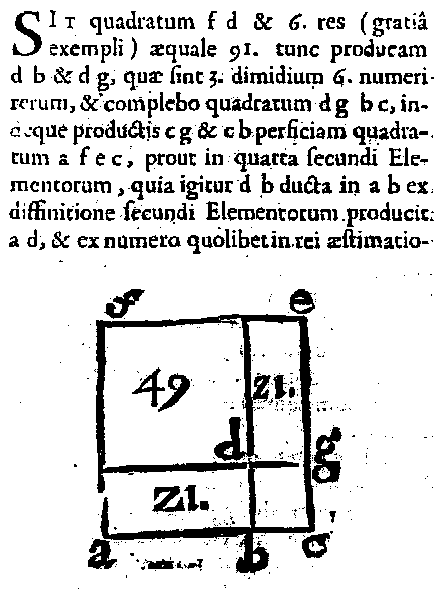
\includegraphics[width=\linewidth]{cardano-quad}
\end{minipage}
\goodbreak


\begin{minipage}[t]{0.65\linewidth}\vspace{0pt}
	The quadratic algorithms were well-established by this time; on the following page of his text, we find a picture from the work of al-Khwārizmī (Exercise \ref*{sec:islamalgebra}.\ref{exs:alkalgebra}), after which comes more obvious mathematical notation. Even though Rudolff's $\pm$ and $\sqrt{}$ were in use, Cardano wrote almost everything in words augmented with fractional notation and Pacioli's $\cl p$ and $\cl m$.\smallbreak
	As was typical for the time, Cardano describes negative solutions as fictitious; he even writes the square root of $-15$ at one point, though only to mention its absurdity. He also follows the Islamic approach of solving a concrete problem of each type rather than proceeding abstractly, though observe the \emph{gratia exempli} (``for the sake of an example'') as acknowledgement that the general problem $x^2+ax=b$ may be solved identically.\medbreak
	It is for the solution of cubic (and quartic) equations that Cardano is most famous. Below we describe, in modern notation, Cardano's method for solving the cubic equation $x^3+bx=c$ where $b,c>0$, though we stress (again) that Cardano only gave \emph{examples} not a general formula.
\end{minipage}
\hfill
\begin{minipage}[t]{0.32\linewidth}\vspace{-5pt}
	\flushright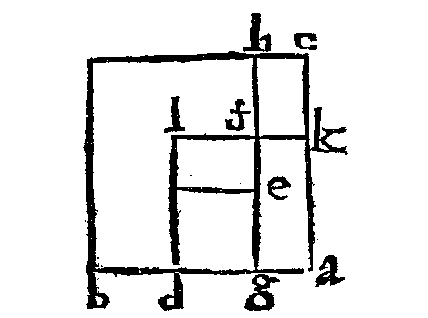
\includegraphics[width=\linewidth]{cardano3}\par
	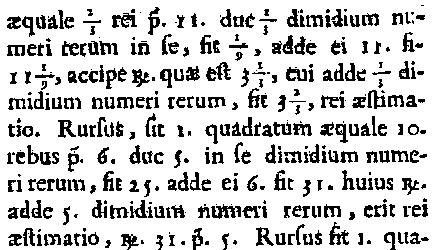
\includegraphics[width=\linewidth]{cardano2}
\end{minipage}\par


\begin{quote}
	Let $u,v$ satisfy $u^3-v^3=c$ and $uv=\frac{b}{3}$.
	Then $x=u-v$ is seen to solve the cubic.
	\begin{align*}
		x^3+bx&=(u-v)^3+b(u-v)=u^3-3u^2v+3uv^2-v^3+b(u-v)\\
		&=(u^3-v^3)+(u-v)(b-3uv)=c
	\end{align*}
	However $u$ and $v$ also satisfy
	\[
		(u^3+v^3)^2=(u^3-v^3)^2+4(uv)^3=c^2+4\left(\frac{b}{3}\right)^3
	\]
	so we obtain a system of linear equations in the unknowns $u^3,v^3$ which are easily solved:
	\begin{gather*}
		\begin{cases}
			u^3+v^3=\sqrt{c^2+4\left(\frac{b}{3}\right)^3}\\
			u^3-v^3=c
		\end{cases}
		\implies
		\begin{cases}
			u=\sqrt[3]{\sqrt{\left(\frac c2\right)^2+\left(\frac{b}{3}\right)^3}+\frac c2}\\
			v=\sqrt[3]{\sqrt{\left(\frac c2\right)^2+\left(\frac{b}{3}\right)^3}-\frac c2}
		\end{cases}
		\\
		\implies x=u-v
		=\sqrt[3]{
			\sqrt{\left(\frac c2\right)^2+\left(\frac{b}{3}\right)^3} +\frac c2
		}
		-\sqrt[3]{
			\sqrt{\left(\frac c2\right)^2+\left(\frac{b}{3}\right)^3} -\frac c2
		}
	\end{gather*}
\end{quote}

\boldinline{Examples}
\exstart We apply Cardano's method to $x^3+6x=7$, which has the obvious solution $x=1$.
	\begin{align*}
		\begin{cases}
			u^3-v^3=7\\
			uv=\frac 63=2
		\end{cases}\ 
		&\implies (u^3+v^3)^2=7^2+4\cdot 2^3=81 \implies u^3+v^3=9\\[-5pt]
		&\implies u^3=\frac 12(9+7)=8,\qquad v^3=\frac 12(9-7)=1\\
		&\implies x=u-v=\sqrt[3]{8}-\sqrt[3]{1} =2-1=1
	\end{align*}

\begin{enumerate}\setcounter{enumi}{1}
  \item This time we solve $x^3+3x=14$.
	\begin{align*}
		\begin{cases}
			u^3-v^3=14\\
			uv=\frac 33=1
		\end{cases}\ 
		&\implies (u^3+v^3)^2=14^2+4\cdot 1^3=200 \implies u^3+v^3=10\sqrt 2\\[-6pt]
		&\implies
		\begin{cases}
			u^3=\frac 12(10\sqrt 2+14)=5\sqrt 2+7 =(\sqrt 2+1)^3\\
			v^3=5\sqrt 2-7=(\sqrt 2-1)^3
		\end{cases}\\
		&\implies x=u-v=(\sqrt 2+1)-(\sqrt 2-1)=2
	\end{align*}
	As this shows, Cardano's formula might produce an ugly expression for a simple answer. And, of course, the cube root of $5\sqrt 2\pm 7$ is something that's on the tip of everyone's tongue!
	
	\item The equation $x^3+3x=10$ may be solved using Cardano's method, though in this case the answer is just ugly.
	\begin{align*}
		\begin{cases}
			u^3-v^3=10\\
			uv=\frac 33=1
		\end{cases}\ 
		&\implies (u^3+v^3)^2=10^2+4\cdot 1^3=104 \implies u^3+v^3=2\sqrt{26}\\[-3pt]
		&\implies u^3=\sqrt{26}+5,\qquad v^3=\sqrt{26}-5\\
		&\implies x=u-v=\sqrt[3]{\sqrt{26}+5}-\sqrt[3]{\sqrt{26}-5} \approx 1.6989
	\end{align*}
\end{enumerate}


\bigbreak


Being unable or unwilling to work directly with negative numbers, Cardano modified his method to solve other cubics such as $x^3+c=bx$, and moreover described how to remove a quadratic term from a cubic using what is now known as the \emph{Tschirnhaus substitution} ($x=y-\frac a3$):
\[
	x^3+ax^2+bx+c =\left(y-\frac a3\right)^3+a\left(y-\frac a3\right)^2+b\left(y-\frac a3\right)+c =y^3-\frac{a^2}3y+\cdots \tag{$\ast$}
\]
Cardano's student, Lodovico Ferrari, extended the method to solve quartic equations in terms of the solution of a resultant cubic.

\goodbreak

\boldsubsubsection{Negative Solutions and Complex Numbers}

By the late 1500s, mathematicians were mentioning negative solutions to equations---these were usually described as \emph{fictitious,} or \emph{false roots,} but this didn't stop them from being investigated. Rafael Bombelli (1526--1572, Rome) even introduced a notation for complex numbers, described their algebra, and showed how they could be used to find solutions to any quadratic or cubic equation. For instance, he wrote $4+3i$ and $4-3i$ as follows:
\begin{quote}
	$4\ p\ di\ m\ 3$, \ read `\emph{quattro piu di meno tre}' (four plus of minus three), and,\\
	$4\ m\ di\ m\ 3$, \ `\emph{quattro meno di meno tre.}'
\end{quote}
Given Bombelli's belief in the fictitiousness of complex numbers, the effort he expended in their honor is extraordinary: this is a prime example of pure abstraction, math for the sake of math!\medbreak

In modern language, the three roots of Cardano's cubic $x^3+bx=c$ are
\[
	u-v,\quad \zeta u-\zeta^2v,\quad \zeta^2u-\zeta v
\]
where $\zeta=e^{2\pi i/3} =\frac{-1+\sqrt 3i}2$ is a primitive cube root of unity. Together with the Tschirnhaus substitution $(\ast)$, Cardano's formula therefore solves all cubic equations.

\goodbreak


\boldinline{Examples}

\exstart Returning to one of our previous examples, if $x^3+3x=14$, then $u=\sqrt 2+1$ and $v=\sqrt 2-1$, from which the three solutions are
\begin{gather*}
	u-v=2\\
	\zeta u-\zeta^2v=(\sqrt 2+1)\frac{-1+\sqrt 3i}2-(\sqrt 2-1)\frac{-1-\sqrt 3i}2 =-1+\sqrt 6i\\
	\zeta^2u-\zeta v=(\sqrt 2+1)\frac{-1-\sqrt 3i}2-(\sqrt 2-1)\frac{-1+\sqrt 3i}2 =-1-\sqrt 6i
\end{gather*}

\begin{enumerate}\setcounter{enumi}{1}
  \item To find a solution to $x^3+\textcolor{red}{3}x^2=3$, we perform the Tschirnhaus substitution $x=y-\frac{\textcolor{red}{3}}3=y-1$ before applying Cardano's method:
	\begin{align*}
		y^3-3y^2+&3y-1+3(y^2-2y+1)=3\implies y^3-3y=1 \tag{$b=-3$, $c=1$}\\
		&\implies
		\begin{cases}
			u^3-v^3=1\\
			uv=-\frac 33=-1
		\end{cases}
		\implies (u^3+v^3)^2=1^2+4(-1)^3=-3\\
		&\implies u^3+v^3=\sqrt 3i \implies u^3=\frac 12(\sqrt 3i+1),\quad v^3=\frac 12(\sqrt 3i-1)\\
		&\implies x=u-v-1=\sqrt[3]{\frac{\sqrt 3i+1}2}-\sqrt[3]{\frac{\sqrt 3i-1}2}-1 
	\end{align*}
	This is ugly! If you know Euler's formula and you choose a compatible pair of cube roots (you need $uv=-1$), this will evaluate to one of three real numbers: the positive solution is in fact $x=2\cos\ang{20}-1\approx 0.8794$.
\end{enumerate}

\goodbreak


\boldsubsubsection{Factorization \& the Fundamental Theorem of Algebra}

By the late 1500s, Viète's abstraction allowed him to streamline Cardano's methods. He also investigated the relationship between the coefficients of a polynomial and its roots. For Viète the roots had to be positive, but later improvements by Thomas Harriot and Albert Girard (1629) applied this to all polynomials with any roots. For instance, if $ax^2+bx+c=0$ has roots $r_1,r_2$, then
\[
	(r_1-r_2)\bigl(a(r_1+r_2)+b\bigr) =a(r_1^2-r_2^2)+b(r_1-r_2)= \bigl(ar_1^2+br_1+c\bigr)-\bigl(ar_2^2+br_2+c\bigr) =0
\]
Provided the roots are distinct,\footnote{In fact the formulas hold even when $r_1=r_2$.} we conclude that
\[
	\frac ba=-(r_1+r_2),\quad
	\frac ca=-r_1^2-\frac bar_1=-r_1^2+(r_1+r_2)r_1=r_1r_2
\]
These are the quadratic version of what are known as Viète's formulas; other versions exist for every degree. Their use amounts to an early form of factorization.


\boldinline{Example}

To solve $3x^2-2x-1=0$, first spot that $r_1=1$ is a root. By Viète's formulas,
\[
	r_1+r_2=-\frac ba=\frac 23\implies r_2=-\frac 13
	\quad\text{or alternatively}\quad
	r_1r_2=\frac ca=-\frac 13\implies r_2=-\frac 13
\]
Think about the relationship between this approach and factorization!\medbreak

A nice side-effect is a method for obtaining the quadratic formula by solving a pair of simultaneous equations analogous to Cardano's cubic approach:
\[
	\begin{cases}
		r_1+r_2=-\frac ba\\
		r_1-r_2=\sqrt{(r_1+r_2)^2-4r_1r_2}=\sqrt{\left(\frac ba\right)^2-4\frac ca}
	\end{cases}
	\implies r_1,r_2=-\frac b{2a}\pm\frac 12\sqrt{\left(\frac ba\right)^2-4\frac ca}
\]
Viète's formulas were central to the later development of Galois Theory (1830) and the Abel--Ruffini theorem regarding the insolubility of quintic and higher-degree polynomials.\medbreak

The remaining key results regarding solutions of polynomials also appeared around this time:
\begin{description}\phantomsection\label{pg:factorthm}
	\item[Fundamental Theorem of Algebra] Including multiplicity, a degree $n$ polynomial has $n$ complex roots. Girard offered the first version in 1629, though a complete proof didn't appear until the work of Argand, Cauchy and Gauss in the early 1800s.
	\item[Factor Theorem] In 1637, Descartes proved that $p(r)=0\Longleftrightarrow p(x)$ is divisible by $x-r$.\par
For instance, to find the roots of $p(x)=x^3+2x^2-13x+10$, Descartes would observe:
	\begin{itemize}
	  \item $p(1)=0\Longrightarrow x-1$ is a factor; use long-division to obtain $p(x)=(x-1)(x^2+3x-10)$.
	  \item $q(x)=x^2+3x-10$ has $q(2)=0$; divide to get $q(x)=(x-2)(x+5)$.
	  \item The roots of $p(x)$ are therefore 1, 2 and $-5$ (Descartes called this last a \emph{false root}).
	\end{itemize}
\end{description}

\goodbreak


\begin{exercises}{}{}
	\exstart Find Viète's formulas for the polynomial $p(x)=x^3+ax^2+bx+c$ with roots $r_1,r_2,r_3$; that is, find the coefficients $a,b,c$ in terms of the roots.\vspace{-10pt}
	
	\begin{enumerate}\setcounter{enumi}{1}
	  \item[](\emph{Hint: By Descartes' factor theorem, $p(x)=(x-r_1)(x-r_2)(x-r_3)$, now multiply out\ldots})
	  
		\item%[14-6]*
	  Solve $x^3-6x^2+9x-4=0$ using Girard's method: first, determine one solution by inspection, then use Viète's formulas to investigate the relationship between the remaining roots.
			
		\item\begin{enumerate}
		  \item Apply Cardano's method to the equation $x^3+6x=20$.\par
		  (\emph{Hint: to finish, compute $(1+\sqrt 3)^3$})
			\item If $b,c>0$, Cardano's method finds a single positive solution to $x^3+bx=c$. Explain why such an equation always has exactly one real solution which is moreover positive.
		\end{enumerate}
		
		\item%[12-28*]
		Prove that if $t$ is a root of $x^3=cx+d$, then
		\[
			r_1=\frac t2+\sqrt{c-\frac{3t^2}4}
			\quad\text{and}\quad 
			r_2=\frac t2-\sqrt{c-\frac{3t^2}4}
		\]
		are both roots of $x^3+d=cx$. Use this to solve $x^3+3=8x$.
		
	
		\item%[14-4]*
		Consider the cubic equation $aaa-3raa+ppa=2xxx$ (as written by Harriot). Show that the substitution $a=e+r$ reduces this to an equation without a square term.\par
		As an example, reduce the equation $aaa-18aa+87a=110$ to a cubic in $e$ without a square term. Find all three solutions in $e$ and therefore find the solutions to the original equation in $a$.
		
		
		\item Find all roots of the cubic $p(x)=2x^2-3x^2-3x+2$ using Descartes' factor theorem.
	  
		
		\item (If you are very comfortable with complex numbers)\lstsp Use Euler's formula to verify that the equation $x^3+3x^2=3$ has the positive solution $x=2\cos\ang{20}-1$. It also has two negative real solutions: find them! 
	\end{enumerate}
\end{exercises}

\clearpage


% \subsection*{Perspective}
% 
% Drawing convincingly in perspective is difficult without math! I.e. how small should one draw an object if one knows how far away it is?
% 
% Earliest systematic approaches Brunelleschi (1377--1446) and Alberti (1404--1472). Alberti's approach: how to represent squares on the ground on a canvas? Then use this as a coordinate system to plot other objects.
% 
% Suppose a canvas is placed with its base at $(0,0)$. The eye is place a distance $d$ behind and $h$ above the canvas (at $(-d,h)$). Suppose lengths of 1 are marked out on the ground beyond the canvas. The line joining the eye and the point $(a,0)$ has equation]
% \[y=\frac{-h}{a+d}(x-a)\]
% which intersects the canvas a distance $y=\frac{ah}{a+d}$ from the base. Alberti then insisted that straight lines on the ground must be represented as straight lines on the canvas. If one has squares perpendicular to the canvas, these will appear to recede towards a vanishing point $V$ at the top middle of the canvas.
% 
% Suppose now that the canvas is twice as wide as the distance from the eye. Rotating through $90^\circ$, it so happens that the straight lines joining the base points to the corner of the canvas are exactly those of the lines of sight. This can be used to plot out the squares.
% 
% \paragraph{Example}
% 
% A road of width 2 recedes into the distance straight ahead of the observer. A `canvas' is placed at the center of the road with width 6 and height 3 and the observer stands a distance 3 behind the canvas at height 3. Draw the road.\\
% Now imaging that a row of telephone poles runs down the left side of the road, each having height 1 and being separated by a distance of 2. Draw the poles.\\
% (Mark distacnes of 1 along the road first and note that first pole has height 1 and that their tops also reced to the vanishing point).
% 
% Cah check that if $(x,y)$ is a co-ordinate system in the plane, then this point gets mapped to the point
% \[(X,Y)=\left(\frac{dx}{y+d},\frac{hy}{y+d}\right)\] 
% on the canvas. Can then prove that circles become ellipses.
% 
% Other methods are available!
% 
% \paragraph{A 3D construction and some theorems}
% 
% How do we know that this is what the eye sees?\\
% 
% Suppose that the $xz$-plane is the canvas, the eye is at $(0,-d,h)$. We consider how to project a point $(x,y,0)$ in the $xy$-plane onto the canvas.\\
% If the co-ordinates of the intersection with the canvas are $(X,0,Z)$, then there must exist $t\in\R$ s.t.
% \[(1-t)\threevec 0{-d}{h}+t\threevec xy0=\threevec X0Z\]
% Clearly $t=\frac d{y+d}$ and
% \[X=\frac{dx}{y+d}\qquad Z=\frac{hy}{y+d}\]
% This is exactly the construction from before. We can even extend to 3D: 
% 
% \begin{thm}
% If $(x,y,z)$ is projected onto the canvas $Y=0$ with the eye at $(0,-h,d)$, then
% \[X=\frac{dx}{y+d},\qquad Z=\frac{hy+dz}{y+d}\]
% If we fix a 3D location plane (e.g. $z=0$), then these projections are invertible:
% \[X=\frac{dx}{y+d},\qquad Z=\frac{hy}{y+d},\qquad x=\frac{hX}{h-Z},\qquad y=\frac{dZ}{h-Z}\]
% This transform in 3D is not invertible, since many points are mapped to the same location.\\
% A line in 3D is projected to a line on the canvas.\\
% A conic curve in 3D (quadratic planar curve) is projected to a conic on the canvas.\\
% Parallel lines which are parallel to the plane $z=0$ project to lines that meet at the top of the canvas.
% \end{thm}
% 
% \begin{proof}
% One can compute these facts directly. For the line concept, take two points on the line, then the plane joining these and the eye is ruled by the sight-lines, whence its intersection with the canvas (also a line) is the image of the original line.\\
% For the quadratic, suppose that $q(x,y,z)=0$ is a quadratic form. Intersect with a plane and one obtains a quadratic in two variables (elminate $z$). This defines a cone from the eye, which necessarily intersects the canvas in a conic.\\
% Suppose that two lines are parameterizes by $P+t\vv$ and $Q+t\vv$ where $v_3=0$. Compute that the $(X,Z)$ co-ordinates in the limit as $t\to\infty$ are
% \[X\to\frac{dv_1}{v_2},\qquad Z\to h+\frac{dv_3}{v_2}=h\]
% The $X$-coordinate depends only on the vector $\vv$.
% \end{proof}
% 
% For drawing, say a staircase, this amounts to the 2-point perspective method.
% 
% Weirdly the conic can change type.
% 
% \paragraph{Example}
% 
% Suppose that $d=1=h$. Draw the circle $x^2+(y-r)^2=r^2$ for different values of $r$.\\
% 
% If $h,d$ are fixed, what planar curve corresponds to the circle $X^2+(Z-\frac h2)^2=\frac{h^2}4$?
% 
% The lines $(t,t,1)$ and $(a+t,t,1)$ are parallel. Where do they meet on the canvas? Answer: not on the vanishing line\ldots

%\clearpage



\subsection{Astronomy and Trigonometry in the Renaissance}

Distinctly European progress in trigonometry came courtesy of Johannes Müller (a.k.a.{} Regiomontanus,\footnote{His grand-sounding name is a latinization of his birthplace Königsberg (\emph{King's Mountain}), Bavaria, Germany.} 1436--1476). \emph{De Triangulis Omnimodius} (\emph{Of all kinds of triangles,} 1463) provided an axiomatic update of Ptolemy's \emph{Almagest} and its Islamic improvements. Though the title refers to triangles, his approach remains circle-based (chords and half-chords). Regiomontanus was a renowned astronomer; his tracking of a comet from late 1471 to spring 1472 provided controversial evidence that objects could move between the, supposedly fixed, heavenly spheres of ancient Greek theory.\smallbreak

Domenico Novara (1454--1504), Regiomontanus' student, inherited much of his unpublished work. He became a student of Pacioli in Florence and an astronomer at the University of Bologna, though he is now perhaps best known as adviser to a young Pole, Nicolaus Copernicus (1473--1543), who studied in Bologna from 1496 with the ostensible intent of joining the priesthood\ldots\par

\begin{minipage}[t]{0.69\linewidth}\vspace{-3pt}
	Copernicus concluded that Ptolemy's geocentric model could not be reconciled with astronomical observation. \emph{De revolutionibus orbium celestium} (\emph{On the revolutions of the heavenly spheres}), published a year after his death, describes how to compute within a \emph{heliocentric} (\emph{sun-centered}) model. This, Copernicus believed, was the obvious solution to the problem of \emph{retrograde motion} that had plagued the ancient Greeks.\footnotemark{}\smallbreak
	The animation demonstrates Copernicus' solution: with the sun at the center, the retrograde motion of \textcolor{red}{Mars} and \textcolor{Green}{Jupiter} are easily explained. The \textcolor{orange}{outer circle} represents the `fixed stars' against which the motion of the planets are observed.
\end{minipage}
\hfill
\begin{minipage}[t]{0.3\linewidth}\vspace{-8pt}
	\flushright\href{%
		http://math.uci.edu/~ndonalds/math184/retrograde.html%
	}{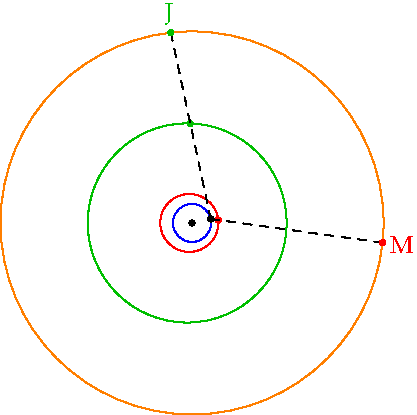
\includegraphics[scale=0.7]{retrograde-movie}}
\end{minipage}\medbreak

\footnotetext{Copernicus wasn't the first to suggest such a model. Several ancient Greek scholars embraced heliocentrism, with Aristarchus of Samos (c.\,310--230\BC) credited with its first presentation. However, Aristarchus' views were rejected by the mainstream Greeks, and it is likely Copernicus never encountered his work.}

% Each step = 3 days\\
% Outer circle = fixed stars\\
% 
% \begin{tabular}{l|l|l|l}
% Planet&Color&Period&Semi-major axis\\\hline
% Earth&Blue&1 year&1 AU\\
% Mars&Red&1.88 years&1.52 AU\\
% Jupiter&Green&11.86 years&5.2 AU
% \end{tabular}


Copernicus' work is now described as a revolution, though it was not perceived so at the time. \emph{De revolutionibus} was dedicated to the Pope, welcomed by the Church, and used by Vatican astronomers to aid in calculation. The difficulty and narrow readership of his work made it unthreatening to contemporary dogma. Copernicus did not present heliocentrism as reality nor did he advocate for overturning long-held beliefs. Within a century, however, the Copernican theory had found its bulldog in Galileo, and conflict between science and the Church became unavoidable.




\begin{minipage}[t]{0.67\linewidth}\vspace{0pt}
	\boldsubsubsection{Trigonometry is finally about triangles!}
	
	Georg Rheticus (1514--1574) defined trigonometric functions purely in terms of triangles, referring to the \emph{perpendiculum} (sine) and \emph{basis} (cosine) of a right-triangle with fixed hypotenuse. Rheticus was a student of Copernicus and helped posthumously to publish his work.\smallbreak
	In 1595, Bartholomew Pitiscus finally introduced the modern term with his book \emph{Trigonometriæ}, in which he purposefully sets out to solve problems related to triangles. The picture is the title page from the second edition (1600---MDC in Roman numerals). Both Rheticus and Pitiscus had problems which look very familiar to modern readers, such as solving for unknown sides of triangles.
\end{minipage}
\hfill
\begin{minipage}[t]{0.32\linewidth}\vspace{-3pt}
	\flushright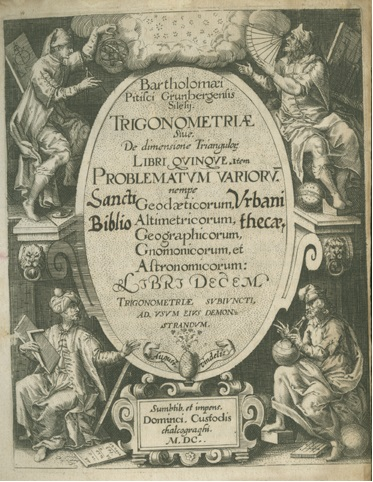
\includegraphics[scale=0.38]{trigonometria}
\end{minipage}\par
\goodbreak



\begin{minipage}[t]{0.58\linewidth}\vspace{0pt}
	\boldinline{Example (Pitiscus)}\phantomsection\label{ex:pitiscus}
	
	A field has five straight edges of lengths 7, 9, 10, 4 and 17 in order. The distance from the first to third vertex is 13 and from the third to fifth is 11. What is the area of the field?\smallbreak
	
	The problem can be solved easily using Heron's formula, but Pitiscus opts for trigonometry. We give a modernized version that depends on applying the law of cosines to the three large triangles.
\end{minipage}
\hfill
\begin{minipage}[t]{0.4\linewidth}\vspace{0pt}
	\flushright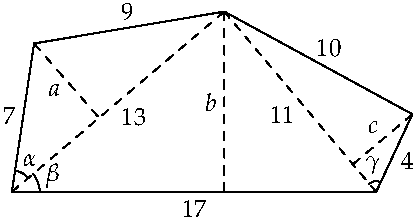
\includegraphics[scale=0.9]{ren-pitiscus}
\end{minipage}\smallbreak

\begin{gather*}
	\cos\alpha=\frac{7^2+13^2-9^2}{2\cdot 7\cdot 13} =\frac{137}{182}\qquad
	\cos\beta=\frac{17^2+13^2-11^2}{2\cdot 17\cdot 13} =\frac{337}{442}\\
	\cos\gamma=\frac{4^2+11^2-10^2}{2\cdot 4\cdot 11} =\frac{37}{88}
\end{gather*}
The values of $\alpha,\beta,\gamma$ and therefore the altitudes $a,b,c$ of the three major triangles could be read off a table, or found exactly using Pythagoras':
\begin{gather*}
	a=7\sin\alpha=7\sqrt{1-\cos^2\!\alpha}=\frac 7{182}\sqrt{182^2-137^2} =\frac 3{26}\sqrt{1595},\\
	b=13\sin\beta=\frac{1}{34}\sqrt{81795},\qquad c=4\sin\gamma =\frac 5{22}\sqrt{255}
\end{gather*}
The total area is easily computed:
\[
	A=\frac 12(13a+17b+11c)=\frac 14\left(3\sqrt{1595} + \sqrt{81795} + 5\sqrt{255}\right) \approx 121.4
\]

\boldsubsubsection{Kepler's Laws}\phantomsection\label{pg:keplerslaws}

Johannes Kepler (1571--1630) was a student of Tycho Brahe\footnote{Tycho Brahe (1546--1601) was a Danish astronomer who worked for Austro-Hungarian Emperor Rudolph II in Prague for 25 years, producing a wealth of accurate astronomical measurements. While these helped burnish the Copernican theory, he is also known for his 1572 observation of a \emph{nova} (a \emph{new} star that later disappeared, now understood to be the death of a distant star), and then a comet in 1577; both provided yet more evidence for the changeability of the heavens.} for the last two years of Brahe's life. He inherited Brahe's position, decades-worth of astronomical data, and his philosophy on the importance of observation-based theory. Kepler also embraced the mystical Pythagorean view that nature reflects harmony, a belief that partly drove his scientific pursuits. To Kepler, any observation of a natural, simple ratio was something of great import. For example, in observing that the daily movement of Saturn at its furthest point from the sun was roughly $4/5$ of that at its nearest point, his temptation was to assume that `roughly' must be `exactly.'\par

\begin{minipage}[t]{0.66\linewidth}\vspace{-3pt}
	Thanks to Brahe, Kepler had data on roughly thirteen orbits of Mars and two of Jupiter. From these data, he posited three laws.
	\begin{enumerate}\itemsep0pt
	  \item Planets move in ellipses with the sun at one focus.
		\item The orbital radius sweeps out equal areas in equal times. In the picture, the sectors all have the same area and the planet moves more slowly the further it is from the sun.
		\item The square of the orbital period is proportional to the cube of the semi-major axis of the ellipse: $T^2\propto a^3$.
	\end{enumerate}
\end{minipage}
\hfill
\begin{minipage}[t]{0.32\linewidth}\vspace{-10pt}
	\flushright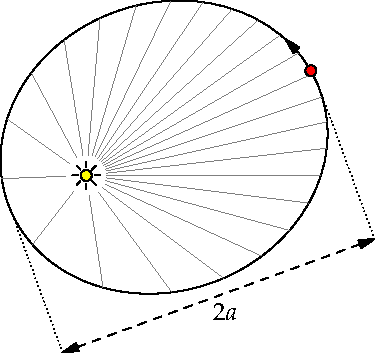
\includegraphics[scale=0.85]{ren-kepler}
\end{minipage}
\goodbreak


Kepler's laws are empirical observations rather than the result of mathematical proof. However, the process of their discovery demonstrates Kepler's tremendous mathematical abilities.

\begin{description}
  \item[Starting point] Kepler began by assuming the essential correctness of the Copernican model in that all planets exhibit uniform circular motion round the sun.\par
	\begin{minipage}[t]{0.65\linewidth}\vspace{-5pt}
  	\item[Orbital Estimation] Kepler's data told him the \emph{direction} to each planet, but not the \emph{distance,} though his Copernican assumption allowed him to estimate the \emph{relative distance}.\footnotemark{} For example, using the direction from \textcolor{Green}{Earth} to \textcolor{red}{Mars} at equally spaced times and by drawing circles of different radii for possible orbits of Mars, he was able estimate an orbit where Mars' motion would also be uniform. This required an enormous number of trigonometric calculations: each measurement of planetary longitude/latitude \emph{relative to Prague} had to be converted to measurements relative to the sun. Everything was subject to errors of estimation.
	\end{minipage}
	\hfill
	\begin{minipage}[t]{0.33\linewidth}\vspace{-6pt}
		\flushright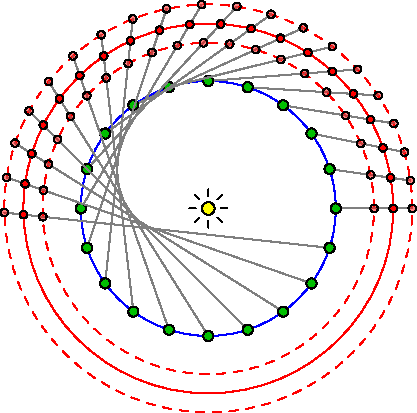
\includegraphics[scale=0.75]{ren-kepler3}
	\end{minipage}\par

  \item[Modifying the model] Kepler altered his model to reflect Earth's slightly non-circular orbit. He first tried an equant model (in the style of the ancient Greeks), offsetting the center of the orbit slightly from the sun. Despite this, he failed to fit his data for Mars to pure circular motion.
  
  \item[The First Law] Abandoning circles, Kepler now permitted planets to move in ovals. He decided to approximate Mars' orbit with an ellipse and set out to calculate its parameters, stumbling on an almost perfect match when the sun was placed at a focus. The \emph{geometric} significance of the focus was exactly the natural beauty sought by Kepler. Having now established the first law for Mars, he repeated the exercise for the other known planets (Mercury, Venus, Earth, Jupiter, Saturn) as well as he could given his inferior data.
  
  \item[The Second Law]\phantomsection\label{pg:kepler2} Kepler's second law followed an infinitesimal argument based on inspired guesswork. To fit his elliptical orbits, planetary velocity was non-constant, appearing inversely proportional to the distance from the sun ($v=\frac kr$). Kepler used this to approximate the area of a sector swept out by the radius vector: over a small time-interval $\Delta t$, a planet travels a distance $v\Delta t$ and thus sweeps out an approximate triangle of area $\frac 12rv\Delta t=\frac 12k\Delta t$. In modern language, this is the conservation of angular momentum. Kepler had no justification beyond the fact that it seemed to fit the data. In particular, he did not know why a planet should move more slowly when further from the sun.
  
  \item[The Third Law] This was stated with very limited analysis. Given the relative sizes of each orbit and its period, some inspired guesswork allowed him to observe that $\frac{T^2}{a^3}$ is approximately the same value for each.
\end{description}

\footnotetext{Following Ptolemy, Brahe thought the Earth-Sun distance was around $1/10$ of its true value. Kepler thought this an underestimate by at least a factor of three. In 1659, Christiaan Huygens found the distance to an accuracy of 3\%.}

Kepler's discoveries were revealed over many years in several texts, and his magnum opus \emph{Epitome astronomiæ Copernicanæ} was published in 1621. Within a century Issac Newton had provided a mathematical justification of Kepler's laws based on the theory of calculus and his own axioms: an inverse square law for gravitational acceleration and his own three laws of motion.

\goodbreak


\boldsubsubsection{A Religious Interlude: Protestantism, the Counter-Reformation and Calendar Reform}

In 1563, Pope Gregory began the Catholic Church's push-back against the spread of Protestantism,\footnote{Martin Luther's \emph{Ninety-five Theses} (1517) is generally considered the start of the Protestant Reformation. Europe saw several gruesome religious wars over the next 150 years as various countries broke from Catholicism and Rome.} the \emph{counter-reformation.} Of particular interest to science and mathematics was the newly created \emph{Index Librorum Prohibitorum,} a list of books contradicting Church doctrine. This was also a response to the new technology of mass-printing, which made disseminating controversial new ideas easier. Heliocentrism came quickly under attack: Kepler's book was banned immediately upon publication in 1621. However, his location far from Rome meant that Kepler and his ideas were relatively safe. The ultimate result of Gregory's crackdown was the slow ceding of scientific power to northern (Protestant) Europe where papal diktat had no effect. \smallbreak

In contrast to the anti-scientific book-banning fervor of the counter-reformation, Pope Gregory is also famous for shepherding an astounding scientific achievement: calendar reform. By 1500, astronomers knew the solar year to be roughly $11\frac 14$ minutes shorter than the $365\frac 14$ days of the Julian calendar.\footnote{Named for Julius Caesar, the Julian year has 365 days with a leap-day added every four years.} For 1200 years, Easter had been decreed to be the Sunday after the first full moon after the vernal equinox (March 20\th/21\st), but by 1500 the equinox was happening 10--11 days earlier. The impetus to correct the date of Easter meant that calendar reform and astronomical modelling were now an important Church project.\smallbreak

A century of effort\footnote{Pope Sixtus IV tried to recruit Regiomontanus to the cause in 1475, though the mathematician died first. Copernicus was among those invited to consider proposals in the early 1500s, though he distanced himself, perhaps because he knew that his developing heliocentric ideas would not be accepted.} resulted in the \emph{Gregorian calendar} (designed by Aloysius Lilius and Christopher Clavius). Gregory imposed the new calendar in all Catholic countries in 1582. The 10 day deficit was corrected by eliminating October 5\th--14\th{} 1582. To prevent the error re-occurring, the computation of leap-years was also changed: centuries are now leap-years only if divisible by 400, thus 1600 was a leap year, but 1900 was not. The Gregorian calendar is astonishingly accurate, losing only one day every 3000 years. Since it emanated from Rome, many Protestant parts of Europe took decades if not centuries to adopt the new calendar. The Eastern Orthodox Church still computes Easter using the Julian calendar, which is now 13 days behind the Gregorian.


\boldsubsubsection{Galileo Galilei (1564--1642)}

Based in northern Italy, Galileo was close to the center of Church power; unlike Copernicus and Kepler, he openly challenged its orthodoxy. While undoubtedly a great mathematician, he is more importantly considered the father of the scientific revolution for his reliance on experiment and observation. He famously observed Jupiter's moons with a telescope of his own invention, noting that objects orbiting an alien body was counter to Ptolemaic theory. Skeptics, when shown this image, preferred to assert that it must be somewhere \emph{inside} the telescope!\smallbreak

In 1632 Galileo published \emph{Dialogue Concerning the Two Chief World Systems,} a Socratic discussion between three characters: Salviati argued for Copernicus, Simplicio was for Ptolemy, and Sagredo was an independent questioner. The character of Simplicio was provocatively modeled on conservative philosophers who refused to consider experiments and bore a notable resemblance to the Pope. Salviati almost always came out on top and Simplicio was made to appear foolish. The text resulted in Galileo's conviction for heresy; all his publications, past and future, were banned, and he spent the remainder of his life under house arrest.\smallbreak

Despite Church efforts, Galileo's works continued to be distributed by his supporters and he continued working. His most important scientific text, \emph{Discourses Concerning Two New Sciences} (materials science and kinematics) was smuggled out of Italy to be published in Holland in 1638. In this book he resurrects his characters from \emph{Two Chief World Systems} and famously refutes Aristotle's claim that heavier objects fall more rapidly than lighter ones.\footnote{Supposedly by dropping weights off the leaning tower of Pisa, though take this story with a pinch of salt\ldots} Here are two results from this text.

\begin{thm*}{}{}
	If acceleration is uniform, then the average speed is the average of the initial and terminal speeds.
\end{thm*}
\phantomsection\label{pg:galileo}

\begin{proof}
	Galileo argues pictorially.\par
	\begin{minipage}[t]{0.8\linewidth}\vspace{-5pt}
		In essence, $\cl{CD}$ is the time-axis, increasing downward. Velocity is measured horizontally from the time-axis to the uniformly sloped line $\cl{AE}$, of which $I$ is the midpoint.\smallbreak
		The distance travelled is the area between $\cl{AE}$ and the time-axis, which plainly equals the area of the rectangle between $\cl{GF}$ and the time-axis. The velocity corresponding to $\cl{GF}$ is the average of those corresponding to $A$ and $E$.\smallbreak
		Here is the calculation using modern algebra. Suppose the object has velocity $v_A$ as it passes $A$ and $v_B$ as it passes $v_B$, and that $t=\nm{AB}$. Then the distance travelled is
		\[
			v_{\text{av}}t =v_At+\operatorname{area}(\triangle ABE) =v_At+\frac 12(v_B-v_A)t=\frac 12(v_A+v_B)t
		\]
		whence $v_{\text{av}}$ is the average of the initial and final speeds.
	\end{minipage}
	\hfill
	\begin{minipage}[t]{0.18\linewidth}\vspace{-20pt}
		\flushright\includegraphics[scale=0.45]{galileo-accel}
	\end{minipage}
\end{proof}

\begin{cor*}{}{}
	A falling object dropped from rest will traverse distance in proportion to time-squared,
	\[
		d_1:d_2=t_1^2:t_2^2
	\]
\end{cor*}

This is Galileo's version of the well-known kinematics formula $d=\frac 12gt^2$.

\begin{proof}
	Let $d_1,d_2,v_1,v_2$ represent the distances travelled and the speeds of the dropped body at times $t_1$ and $t_2$. Since acceleration is uniform,
	\[
		v_1:v_2=t_1:t_2
	\]
	By the Theorem,
	\[
		d_1=\frac{0+v_1}2t_1=\frac 12v_1t_1,
		\quad\text{and}\quad
		d_2=\frac 12v_2t_2
	\]
	whence
	\[
		d_1:d_2=v_1t_1:v_2t_2=t_1^2:t_2^2\tag*{\qedhere}
	\]
\end{proof}

Galileo follows this by decomposing the motion of a projectile into horizontal (uniform speed) and vertical (uniform acceleration) components, thereby proving that projectiles follow parabolic paths.\smallbreak

Galileo covered several other important mathematical topics, some of which we'll mention when we discuss calculus. While his mathematical ideas were cutting-edge for the time, it is his insistence on testing theory against data that makes him a true revolutionary. By 1600 very few of Aristotle's easy-to-refute claims had been rejected due to experimental testing; the hostility Galileo provoked by doing so perhaps explains why. This is the core of the scientific revolution: primacy is given to experiment and observation over ancient `wisdom,' whatever the source.\smallbreak

Galileo was finally cleared of heresy by the Catholic Church in 1992.



\begin{exercises}{}{}
	\exstart \emph{Compute} today's date in the Julian calendar and explain your calculation.
	
	\begin{enumerate}\setcounter{enumi}{1}
		\begin{minipage}[t]{0.7\linewidth}\vspace{3pt}
	 		\item%[13-14]
	 		(A problem of Copernicus)\lstsp Given the three sides of an isosceles triangle, to find the angles.\smallbreak
	  	Suppose $\cl{AB}$ and $\cl{AC}$ are the equal legs of the triangle. Circumscribe a \textcolor{blue}{circle} around the triangle and draw \textcolor{red}{another} with center $A$ and radius $\cl{AD}=\frac 12\cl{AB}$.
			\begin{enumerate}
		  	\item Why is Copernicus introducing the second circle?
		  	\item Explain why the ratio of each of the equal sides to the base of $\triangle ABC$ equals that of the radius $\cl{AD}$ to the chord $\cl{DE}$.
		  	\item If $\nm{AB}=\nm{AC}=10$ and $\nm{BC}=6$, use modern trigonometry to find the three angles of the original triangle.
			\end{enumerate}
		\end{minipage}
		\hfill
		\begin{minipage}[t]{0.28\linewidth}\vspace{3pt}
			\flushright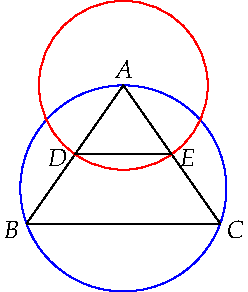
\includegraphics{hw5-copisotri}
		\end{minipage}
	
	  \item Verify that Heron's formula gives the same solution to Pitiscus' problem (pg.\,\pageref{ex:pitiscus}).
	  
	  \item%[13-17]
	  Given that Earth's orbital period is 1 year and that the mean distance of Mars from the sun is 1.524 times that of Earth, use Kepler's third law to determine the orbital period of Mars.
	  
	  \item%[13-18]
	  According to Kepler's second law, at what point in a planet's orbit will it be moving fastest?
	  
	  \item%[13-24]*
	  Galileo states the following.
	  \begin{quote}
	  	A projectile fired at an angle $\alpha=\ang{45}$ above the horizontal at a given initial speed reaches a distance of 20,000. Then, with the \emph{same} initial speed it will reach a distance of 17,318 when $\alpha=\ang{60}$, or $\alpha=\ang{30}$.
	  \end{quote}
	  Check this statement: if you want a challenge, try to do without the standard Physics formulæ and instead use ratios!
	\end{enumerate}
\end{exercises}